\chapter{Machine Learning for Quality Control} \label{Machine Learning for Quality Control}
\minitoc

\section{Introduction}

Recent advancements in Machine Learning in the last few decades have opened up new research perspectives in the quality monitoring domain. In this chapter, we describe a general framework that can be applied to model the relationship between machine process data and product quality. The described methods relies on four consecutive stages: data acquisition, data processing, exploratory data analysis and supervised machine learning modelling. The application of such a method could bring a few major benefits to the manufacturing company: on one side, it would allow for a better understanding of which process parameters have an important influence on finished parts quality. In such a way, it is possible to put them under close monitoring to ensure their stability over time. Moreover, the trained model could be used to infer part quality given a new set of input process data. In such a way it is possible to provide a quality status to each part produced. This is particularly interesting every time that a quality control cannot be performed on all part produced. In fact, most companies cannot test every single product. There may simply be too high a volume or number of them to inspect at a reasonable cost or within a reasonable time frame. Or effective testing might result in the destruction of the product or render it unfit for sale in some way. By providing the quality status for 100\% of the part produced it is possible to react faster to quality non-conformities and to avoid sending to the customer a part which is non compliant with the specifications.  In the second part of the current chapter, we also bring a special attention to define the core concepts and approaches used in Machine Learning, thus serving as an introduction to Machine Learning algorithms and techniques extensively used in the other chapters of this PhD dissertation.

\section{Towards data-driven quality control}

In the manufacturing industry, product quality is an indicator for evaluating the production capacity of a company. Customers are increasingly demanding in terms of product quality and providing the customer with a product that complies with the specifications is absolutely essential in a market that is becoming more and more competitive. The best possible solution to deliver 100\% of compliant parts to the customer would be to inspect in details all parts produced. However, most companies cannot test every single product. There may simply be too high a volume or number of them to inspect at a reasonable cost or within a reasonable time frame. Or effective testing might result in the destruction of the product or render it unfit for sale in some way. In our industrial context, the quality control is a time-consuming operation that requires several minutes of work and that cannot be done online for each part. As a consequence, only a subset of the produced parts can be measured. One set of statistical tools for applying such a screening is acceptance sampling. Using such tools enables decision makers to determine what action to take on a batch of products. Decisions based on frequency testing, rather than on 100\% inspection, are more expedient and cost effective but it cannot guarantee the conformity of all parts of the population from which the sample was drawn~\citep{fuchs1998multivariate}.
% In this section, we extend the concept that was presented in Chapter \ref{From Corrective to Predictive Process Control} in order to develop a general framework for inferring the quality of a manufactured part without directly measuring it. One more time, we will take advantage of machine learning ability to learn the transfer function from some input data to the product quality. The trained model could then be applied to enhance manufacturing quality control by providing a quality status to the part.
Figure \ref{fig:statistical_quality_control} outlines the functioning of acceptance sampling. 

\begin{figure}
\centering
\includegraphics[scale=0.50]{images/chapter_4/statistical_quality_control.png}
\caption{Statistical quality control}
\label{fig:statistical_quality_control}
\end{figure}

Although this method is widely applied in the manufacturing industry and it is globally accepted, it presents three major drawbacks:
\begin{enumerate}
    \item The acceptance sampling method is able to track deviations in product quality, but it is not able to provide 100\% quality inspection. As a result, it may happen that one or multiples non-compliant parts are produced, as a response to a temporary malfunction in the production process, and these parts may not be detected. This may result in one or multiple non-compliant parts being sent to the customer.
    \item The second drawback of Acceptance Sampling is the delay in detecting a process deviation. If product quality starts to deviate, the manufacturer has to wait for the next quality control to identify the problem and to be able to act on the process to correct it. Moreover, parts produced in this time frame are potentially non-compliant and extra time-consuming quality control may be required to establish whether or not the parts can be sent to the customer.
    \item Another problem to consider, is the one related to the destruction of the pieces being measured. In fact, some quality measurements involve the destruction of the part or some modifications that make it unsuitable for sale to the customer. For instance, advanced quality control for assessing material distribution of each thickness layer of a blow-moulded part requires the cutting of the piece in small samples, subsequently analysed in the laboratory. Even if these tests are necessary and important to certify partconformity, it constitutes a source of waste for the manufacturer, increasing the number of PPM (parts per million) defects.
\end{enumerate}
%
In order to improve quality control of the parts, we propose to perform a comprehensive quality control using a machine learning based approach. The idea is to infer the quality status of each part produced through the use of a machine learning algorithm. The approach would be described in details in the following sections of the current chapter. 
In the context of this PhD study, the approach of inferring part quality using a trained machine learning algorithm is called \textit{data driven model-based quality control}.
The benefits that this approach can bring to quality control throughout the manufacturing industry are manifold. First, it ensures a quality control on all parts produced which enable for a fast reaction to quality non-conformities (Figure \ref{fig:model_quality_control} on the left side). In fact, by ``virtually'' measuring each part, we are able to eventually discard parts for which the model has provided a ``Not-OK'' result, or request the quality team to carry out more in-depth tests. Model-based quality measurement may be effectively used to detect those parts that turn out to be, from a statistical point of view, outliers. In this way, instead of randomly sampling the parts to be measured by the quality operators, the model is able to suggest parts that seem to be interesting.
By discarding all non-compliant parts, this approach indirectly reduces product recalls and thus the whole series of requests to return, exchange or replace a product that has been found to be defective, and which could impair performance, harm consumers or cause legal problems for producers.

\begin{landscape}
\begin{figure}
\centering
\includegraphics[scale=0.50]{images/chapter_4/data_driven_model.png}
\caption{Data-driven model-based quality control}
\label{fig:model_quality_control}
\end{figure}
\end{landscape}

If the trained model is sufficiently robust and accurate at predicting the quality status of a part, a second stage would be to reduce the real quality controls which destroy the parts or make them unusable (Figure \ref{fig:model_quality_control} on the right side). In such a case, not only the model-based control would be able to provide a thorough quality control, but it would also be able to reduce the scraps which account for an overall better production performance. Of course, real part measurements cannot be completely replaced by model-based measurements. In fact, real measurements are the primary data source to train the data-driven model. 


\section{Proposed method} \label{Proposed Method}

In this section, we will try to describe a general framework that can be applied to improve process control. We use supervised machine learning to discover some patterns between process parameters and part quality that has been manufactured by the same process. We proceed in four main stages:
\begin{enumerate}
    \item \textit{Data collection} consists in retrieving all the data needed to model the manufacturing production process. It involves two main stages:  data acquisition and  data labelling (Section \ref{Data Collection}). 
    \item \textit{Data processing} covers the range of operations required to make the input data suitable for the machine learning algorithm (Section \ref{Data Processing}). 
    \item \textit{Exploratory data analysis} is an ensemble of graphical and quantitative techniques that can be used to explore data and retrieve important information (Section \ref{Exploratory Data Analysis}).
    \item \textit{Data modelling} corresponds to the statistical modelling of the relationship between the process data and the quality data by a machine learning algorithm (Section \ref{Machine Learning modeling})
\end{enumerate}

In the remaining part of the current section we will review in details how to carry out these four steps to achieve a \textit{predictive process control}. 

\subsection{Data collection} \label{Data Collection}

Collecting data allows to capture a record of past events so that we can use data analysis to find recurring patterns. In the context of this research work, data collection is the task of retrieving the data that could be meaningful to explain the variability of a quality characteristic given some process parameters. Among the many challenges in Industry 4.0, data collection is becoming one of the critical bottlenecks. It is known that the majority of the time for building end-to-end data-driven models is spent on preparing data, which includes collecting, cleaning, analysing, visualising, and feature engineering. Moreover, as machine learning is used in new applications, it is usually the case that there is not enough training data. Traditional applications of machine learning like machine translation or image object detection rely on huge quantities of training data that have been accumulated for decades. On the other hand, more recent applications, especially in the manufacturing industry, have little or no training data. To train a machine learning model, it is necessary to have samples that are representative of the entire operating range of the process. If the individuals do not cover the whole process functioning, the model will be biased.

Two kind of data are required: input data, corresponding to the process data and output data which is actually the measurement of the part quality. Data collection involves mainly two different steps: \textit{process data acquisition} and \textit{Quality data acquisition}. 

\subsubsection{Process data acquisition} \label{Process Data Acquisition}

We use here the term \textit{process data} for any type of data belonging to the manufacturing process. For instance, some process data of the extrusion blow-moulding process are extruder throughputs, extruder temperatures, or blowing air pressures. This process data is a picture of the process state at a given time.

Process data acquisition is a challenging task in Industry 4.0 due to different technologies, machines, sensors, IoT devices and communication networks. Sensors, actuators, and Programmable logic controllers (PLCs) are the main data generators in the automotive industry \citep{khan2017big}. In the last decade a new type of intelligent sensor, also called \textit{smart sensors}, is more and more used in the manufacturing industry. Most of the data available in the Manufacturing plants comes from PLCs, sensors and smart sensors. The three devices are further explained as below.

\begin{itemize}
    \item \textit{Sensors} convert a physical state or activity into an electrical signal that is sent to the PLC for further processing. In manufacturing, sensors create a huge amount of data. Most machines and robots include sensors that collect data from their surroundings, such as temperatures of machine components or its environment.
    \item \textit{Smart sensors} are devices that take information from a physical environment and use embedded microprocessors and wireless communication to monitor, examine and provide information about the proper functioning of the observed system. With the developments of IoT and machine learning, various types of smart sensors are nowadays available.
    \item \textit{Actuators} controlled by the PLC, produce a physical action. A basic example of an actuator connected to a PLC is the automatic starting of a motor. There are several robots for automated procedures in the industry. These robots are actuators that produce a large amount of data.
    \item \textit{PLC} is a programmable unit that takes input from sensors, and controls actuators (Figure \ref{fig:plc}). A factory has has a large number of PLCs which controls the machines. PLCs are manufactured by different suppliers and they generate heterogeneous data which is a big challenge for industrial big data.
\end{itemize}

\begin{figure}
\centerline{\includegraphics[scale=1]{images/chapter_3/PLC.jpg}}
\caption{Programmable logic controller \textit{Siemens} S7-1500}
\label{fig:plc}
\end{figure}


The presented devices produce a lot of data but they do not manage data storage. In fact, PLCs have a limited amount of storage space and they cannot be used to store data permanently. The local machine data storage is most of the time handled by the SCADA (Supervisory Control And Data Acquisition) software. The term SCADA is used to identify any kind of software, installed on a personal computer or server, which allows the implementation, operation and management of supervisory, control and remote control systems without necessarily having to write code using programming languages. SCADA software have multiples functionalities which range from automation, to alarm handling, logging, archiving and simple statistical analysis \citep{daneels1999scada}. SCADA is a powerful system for acquisition of industrial automation data but, it is not able to handle the storage of a large volume of data. For this reason the collected data through SCADA system should be stored elsewhere, in a place where data are easily accessible. Cloud platform, whether they are internal the manufacturing company or outside, are generally the solution for storing a large amount of data. Cloud platforms, or \textit{data Lake}, has been designed to be highly scalable and it provides a way to easily access data through Big data technology that facilitate and accelerate data analysis stages.  

In order to be able to properly manage data acquisition, taking into account the heterogeneity of data coming from the different data sources, we propose to introduce a \textit{Gateway} system which constitutes an intermediary bridge between the shop floor PLCs, sensors, and the Cloud platform where data are stored. Moreover, it can communicate with the \textit{MES} system. The Manufacturing Execution System (MES) is a production management system serving as the information center in the enterprise to improve manufacturing transparency. It is the middle layer connecting the manufacturing process on the shop floor and the business process on the Enterprise Resource Planning (ERP) \citep{chen2020implementation}. By communicating with the MES system, it is possible to associate to a produced part the set of events that have enabled its production.

The architecture of the overall data acquisition system is visible in Figure \ref{fig:data_acquisition_architecture}.

\begin{landscape}
\begin{figure}
\centering
\includegraphics[scale=0.5]{images/chapter_3/Data_acquisition_architecture.png}
\caption{Data acquisition architecture}
\label{fig:data_acquisition_architecture}
\end{figure}
\end{landscape}

The gateway is a physical or virtualized server which acts like an intermediary between data acquisition systems available in the shop floor and Cloud platform where data are stored for data analysis. The gateway is connected to the shop floor network and it is able to interact directly with machine PLCs as well as smart sensors.  

The gateway has two main roles:

\begin{itemize}
    \item It allows to centralize the data collection at plant level. It is in charge to retrieve data from all data sources, whether they are PLCs, smart sensors, SCADA software or the MES system. This process facilitates the subsequent sending of data to the Cloud platform. 
    \item This gateway is well suited for eventually deploying in production at the plant side the machine learning models that have been trained. 
\end{itemize}

The gateway should be equipped with different tools and software to allow the communication with machines through different communication protocols mainly used in Industry 4.0. There exist a multitude of communication protocols. Among all these we can mention \textit{OPC UA} and \textit{MQTT}. OPC UA (Open Platform Communications Unified Architecture) is a service-oriented machine-to-machine communication protocol mainly used in industrial automation. Its main goals are to provide a cross-platform communication protocol while using an information model to describe data transfer \citep{profanter2019opc}. MQTT (Message Queuing Telemetry Transport) is an open message protocol which mainly focuses on a small code footprint and low network bandwidth usage, while handling high latency or bad network connections \citep{profanter2019opc}. Further information regarding communication protocols used in Industry 4.0 are available in \citep{profanter2019opc}\citep{8262021}\citep{zezulka2018communication}.


\paragraph{Process data types}

When dealing with process data, we distinguish two different types of data: \textit{Cyclical data} and \textit{Time series data}.

\begin{itemize}
    \item \textit{Cyclical data}: Cyclical data are scalar values which provide information about a certain recurring event. Examples of Cyclical data are the machine cycle time, or the time needed from the machine to perform an operation. 
    \item \textit{Time series data}: Whenever a production process, or a part of it, requires time to be completed, it is possible to recover multiple sequential values of the same process parameters. This sequence of sequential data take the name of time series. The number of sequential values composing the time series depends on the sampling rate and may change accordingly to the nature of the measurement. For instance, temperature of a machine components may be measured all along the production cycle and it is a classical example of time series data.
\end{itemize}

\begin{figure}
\centering
\includegraphics[scale=0.5]{images/chapter_3/time_series_data.png}
\caption{Time series data}
\label{fig:time_series_data}
\end{figure}


\subsubsection{Quality data acquisition}

Quality data acquisition is the task of collecting product quality data associated with all or some of the parts produced. The quality label can be continuous or discrete depending on the applied measurement method. For instance, we can measure a thickness of a manufactured part and provides the results in the form of continuous values in meters. On the other hand, we can measure a thickness value and associate it to  a class according to its compliance, or non-compliance with the specifications. Accordingly to the type of the label, either discrete or continuous, data modelling may change. If the label is discrete the supervised learning modelling takes the form of a Classification problem (\ref{Classification}), otherwise it will be treated as a Regression problem (\ref{Regression}).   

The quality data acquisition can be done offline or online. The following two paragraphs will provide an overview of these two methods. 


\paragraph{Offline acquisition}

Offline acquisition, is the most common approach for labelling manufacturing data. In fact, for all non-visual product characteristics, it is extremely complicated to assess part quality in less then a minute. Most of quality controls realized on the part require specific equipment and the task of controlling it can take several minute. Moreover, effective controlling might result in the destruction of the product or render it unfit for sale in some way. In such a case, the only possibility is to measure the part quality offline. Measuring offline has the advantage of allowing careful control of the manufactured parts, reducing the possibility of measurement error. However, as there are only a few parts to measure, it may takes a long time to build a dataset which is representative of all categories of part non-compliance.

Since, we are not able to measure the quality of all parts produced, it becomes crucial to structure data collection to make them easily usable for future data analysis. Data have to be stored in a database and  measurement quality must be related to a part number, or traceability number, in order to subsequently associate it with process data, which in turn must be tagged with the part number. 


\paragraph{Online acquisition}

Performing online data acquisition, on production line, eliminates two critical error risks:
\begin{enumerate}
    \item The loss of the link between production measurements and off-line annotation.
    \item The transformation of parts between their production and their annotation.
\end{enumerate}

On the other hand, the time available for annotation is very limited. Most of the time machine operators have time constraints to meet production rate. As a consequence this data annotation must be done in a limited amount of time. The time available  to perform a control may change depending on the operator task. We estimate that the operator can affect a maximum of one third of the production cycle time to this task, which means that for a process with a cycle time of 60 seconds the operator has at maximum 20 seconds to perform it. In addition to the annotation time, the human expert has to assist in the handling of the parts and related operations.

By automating the process data acquisition through the data collection presented above, and by ensuring the proper registration of data quality  obtained by measuring the parts, it is possible to permanently feed a dataset with new data in an automatic manner. Over time we can hope to recover enough data to cover all distribution of all possible quality non-conformities. 

\subsection{Data processing} \label{Data Processing}

As heterogeneous data is collected in manufacturing processes, it becomes necessary to process these data to make them more suitable for data analysis. In general, Data processing is the result of three major tasks: data cleaning, reduction, and scaling.

\begin{itemize}
    \item \textit{Data cleaning} aims to enhance the quality of the data by missing value imputations and outlier removals. 
    \item \textit{Data reduction} is applied to reduce data dimensions and therefore, reducing the computational costs associated. 
    \item \textit{Data scaling} aims to transform the original data into similar ranges for predictive modelling. 
\end{itemize}

In the remaining part of this section we will provide some additional elements regarding these three data processing tasks. 
  
\subsubsection{Data cleaning}

% Missing literature references

Data cleaning is the result of two main operations: missing values imputations and outlier removals.

There are two main approaches to deal with missing data. The first option is to simply reject data samples with missing values since most data mining algorithms cannot handle missing data. This approach is only useful when the amount of missing values is small. The second technique is to use missing value imputation to replace missing data with inferred values. Mean imputation, forward or backward imputation, and moving average techniques are examples of traditional imputation procedures. In such a case, missing values are inferred based solely on the data properties of that variable, and therefore are referred to as univariate techniques. The mean or median imputation method will replace missing values with the mean or median of that variable. The forward or backward method simply replaces the missing value with the previous or next data measurement. More advanced techniques make use of regression model based methods to obtain more accurate imputation results. 

As regarding outlier removals, the most commonly used techniques use statistical analysis to identify which data belongs or not to the data distribution. Data outliers can be identified, for instance, if the data fall beyond a certain range constructed using conventional statistics such as standard deviations, means and quartiles. Identifying outliers is a delicate operation as, what at first glance might appear to be an outlier, could turn out to be extremely interesting data. When dealing with manufacturing process data, the outlier can be representative of a process functioning state which is not normal and could therefore explain some product quality non-compliances. Physical knowledge of the production process is therefore indispensable in order to understand whether the outliers are due to a process malfunction or to a data acquisition error.    


\subsubsection{Data Reduction}

% Missing literature references 

Assuming that data are ranged in a tabular format where the row represents the samples and columns the features, or process parameters, data reduction may be conducted to reduce either the number of samples or the number of columns.
There are three main methods of column-wise data variable reduction: The first is to use domain knowledge to directly select variables of interests. The second is to use statistical feature selection methods to select important variables for further analysis. The third is to adopt feature extraction methods to construct useful features for data analysis.
Human expertise plays a key role in data acquisition process and, globally, in tasks of modelling by statistical learning the relationship between process and product characteristics. For complex process the number of available process parameters are huge, in the order of hundreds and sometimes thousands. The Human experts most of the time have many years of experience working with a particular Manufacturing process and their knowledge of the process may be used to pre-select a number of useful features that can be used to try predicting the target output. 

As regarding feature selection techniques, we distinguish mainly three approaches: the filter, wrapper and embedded methods. The filter method is a simple feature selection approach in which variables are ranked and selected based on specific univariate metrics. Pearson's correlation coefficient is a common filter technique for determining the direction and strength of a linear relationship between two variables. A wrapper method may be used to assess the usefulness of data variables given a certain learning algorithm. Heuristic search methods, such as stepwise forward and backward selection methods, are commonly used. When compared to the filter approach, the wrapper method can take into consideration data variable correlations and interactions with learning algorithms. However, because it is generally performed via an exhaustive search, the computing costs associated with it might be significantly higher. The embedded technique has been developed to optimise the feature selection result via a model training process in order to decrease computation costs. Two popular embedded methods are the L1 regularisation (based on the least absolute shrinkage and selection operator, LASSO) and L2 regularisation (based on ridge regression) (\ref{Parametric models}). By adding the $L1$ or $L2$ regularisation terms to the objective function it is possible to use a penalised linear regression to accomplish the feature selection task.

\paragraph{Stability Selection} \label{Stability Selection}

In our research work we have mostly used the \textit{Stability Selection} method \citep{meinshausen2010stability}.  The main idea behind stability selection is to inject more noise into the original problem by generating bootstrap samples of the data, and to use a learning algorithm to find out which features are important in every sampled version of the data. For a feature to be considered stable (or important), it has to be selected in a high number of perturbed versions of the original problem. This tends to filter out features that are only weakly related to the target variables, because the additional noise introduced by the bootstrapping breaks that weak relationship. The algorithm takes as input a grid of regularisation parameters $\Lambda$, and the number of sub-samples $N$ that need to be generated. Stability selection returns a selection probability $\Pi^{\lambda}_{k}$ for every value $\lambda \in \Lambda$ and for every feature $k$, and the set of stable features $\hat{S}^{stable}\subseteq\{1,…,p\}$. The algorithm consists of two steps. In the sampling step the selection probabilities, or stability scores, are computed as follows. For each value $\lambda \in \Lambda$ do:

\begin{itemize}
    \item For each $i$ in $1,\dots, N$, do:
    \begin{itemize}
        \item Generate a boostrap sample of the original data $X^{n\times p}$ of size $n/2$.
        \item Run the selection algorithm on the boostrap sample with regularisation parameter $\lambda$ to get the selection set $\hat{S}^{\lambda}_{i}$.
    \end{itemize}
    \item Given the selections sets from each sub-sample, calculate the empirical selection probability for each model component:
    \begin{equation}
        \hat{\Pi}^{\lambda}_{k} = \frac{1}{N}\sum_{i=1}^{N}
    \end{equation}
\end{itemize}

In the scoring step we then compute the set of stable features according to the following definition

\begin{equation}
    \hat{S}^{stable} = \{k:\max\Pi^{\lambda}_{k} \geq \pi_{thr}\}
\end{equation}
%
where $\pi_{thr}$ is a predefined threshold. When the stability score for a variable exceeds the threshold $\pi_{thr}$ for one value in $\Lambda$, it is deemed stable. In practice the LASSO penalisation (see section \ref{Parametric models}) is frequently applied to get the selection set $\hat{S}^{\lambda}_{i}$. This is due to the ability of Lasso to performs shrinkage and (effectively) subset selection.


Unlike feature selection, which picks only relevant features from existing variables, feature extraction seeks to create new features based on linear or nonlinear combinations of existing variables. Most common linear feature extraction techniques include principal component analysis (PCA) and statistical methods. Statistical methods typically calculate summarising statistics such as the mean, peak, and standard deviation, for data measurements over a particular time span as features. This approach is particularly suited for time series data. When dealing with time-series data we can compress the entire information in a limited set of new features computed through the use of summarising statistics. When working with PCA, the features extracted, corresponding to the Principal Components, are linear combinations of the original data variables. The PCA-based method can be very useful when there presents data multi-collinearity problem. In practice, the number of principal components or features extracted is determined based on the proportion of total data variance explained, for instance, the principal components should be capable of explaining at least 80 or 90\% of the total data variance. To minimise the potential information loss, more advanced techniques can be applied. Nonlinear feature extraction such as \textit{AutoEncoders} may be used to extract more complex and useful features.


\subsubsection{Data Scaling} \label{Data Scaling}

Data scaling is often needed to ensure the validity of predictive modelling, especially when input variables have different scales. The most used scaling techniques are \textit{max-min normalisation} and \textit{z-score standardisation}. Min-max normalisation is defined as follow:
\begin{equation}
    x = x - x_{min} / x_{max} - x_{min}
\end{equation}

where $x_min$ and $x_max$ refer to the minimum and maximum values of the generic feature x. The z-score standardization is instead defined by the following equation:

\begin{equation}
    x = x - \mu / \sigma
\end{equation}

where $\mu$ is the mean and $\sigma$ is the standard deviation of the feature $x$.

Z-score standardisation is well suited when data are normally distributed.
The max-min normalisation, instead, is recommended when the data do not conform to a normal distribution and have no outliers. 


\subsection{Exploratory data analysis} \label{Exploratory Data Analysis}

Exploratory Data Analysis (EDA) is a set of data analysis techniques that may be applied to:

\begin{itemize}
    \item Uncover underlying structures,
    \item Isolate important variables,
    \item Detect outliers and other anomalies,
    \item Suggest suitable models for conventional statistics.
\end{itemize}

EDA is usually the intermediate stage between Data processing and Data modelling. By exploring the data, it is possible to discover interesting patterns among data and drive the modelling phase depending on what has been observed. Moreover, the EDA allows to fine-tune the Data processing stage. In fact, by exploring the data we can identify useless features that cannot bring any added value and can therefore be discarded.   

The term “Exploratory Data Analysis” was introduced by John W. Tukey who in \citep{tukey1977exploratory} shows how simple graphical and quantitative techniques can be used to explore data.

Typical graphical techniques are:

\begin{itemize}
    \item Plotting the raw data (e.g., stem-and-leaf diagrams, histograms, scatter plots)
    \item Plotting simple statistics (e.g., mean plots, box plots, residual plots)
    \item Positioning (multiple) plots to amplify cognition
\end{itemize}

Typical quantitative techniques are:

\begin{itemize}
    \item Interval estimation
    \item Measures of location or of scale
    \item Shapes of distributions
\end{itemize}

A very convenient tool for performing exploratory data analysis is the Principal Component Analysis (section \ref{Principal Component Analysis}). By projecting input data on Principal Components, it is possible to visualise most of input data variance by simply plotting data to the firsts Principal Components which accounts for the most data variability. In such a way, it is possible to visualise most of the variability of input data, even if the size of the feature space is not negligible. 

\subsection{Machine learning modelling} \label{Machine Learning modeling}

Machine learning modeling involves the use of machine learning algorithm to approximate the transfer function between input process data and output quality data. Mathematically speaking, we look for the function $\hat{f}$ so that:

\begin{equation}
    Q = \hat{f}(X_1,X_2,\ldots,X_p) + \epsilon
\end{equation}

where:

\begin{itemize}
    \item $Q$ is the target quality variable we want to infer given input process parameters.
    \item $\hat{f}$ is the transfer function approximated through the use of a statistical algorithm.
    \item $(X_1,X_2,\ldots,X_p)$ is the set of input process parameters.
    \item $\epsilon$ is an error term which is independent of $(X_1,X_2,\ldots,X_p)$ and which account of the approximation error. 
\end{itemize}

Since we are interested both in prediction and inference, we privilege for this task easily interpretable methods such as parametric models and tree-based methods. 

% rephrase it

The model training is usually done by applying cross validation and hyper-parameter tuning. Different supervised learning algorithms have to be trained and parameterized to allow a comparison of their performances in order to select the best performing model. 

As the a-priori selection of adequate algorithms is not achievable in a generalised way \citep{kotthoff2016algorithm}, different learning methods and algorithms have to be compared and evaluated for each individual application \citep{lee2020machine}. The pre-selection must be made on the basis of selected criteria, e.g. complexity, interpretability, and speed. 
Regarding our use-case of understanding what process parameters affect the most the quality of the manufactured part, the prediction time as well as the potential precision, which is associated with model complexity, are of greater interest. However, algorithm performance is also affected by factors such as data volume. Since we are interested both in prediction and inference, we privilege for this task easily interpretable methods machine learning algorithms such as Parametric models and Tree-based methods and Support Vector Machines. We claims that deep  learning based methods are not well suited for this task as a consequence of their "black-box" nature.

For the evaluation and comparison of model performances, different statistical performance metrics can be applied. For binary classifications, metrics can be calculated based on entries of a confusion matrix, as shown in Table \ref{tab:confusion_matrix}.

\begin{table}[]
\label{tab:confusion_matrix}
\begin{tabular}{l|l|l|}
\cline{2-3}
                                         & Actually Positive              & Actually Negative              \\ \hline
\multicolumn{1}{|l|}{Predicted Positive} & \textbf{True Positives (TPs)}  & \textbf{False Positives (FPs)} \\ \hline
\multicolumn{1}{|l|}{Predicted Negative} & \textbf{False Negatives (FNs)} & \textbf{True Negatives (TNs)}  \\ \hline
\end{tabular}
\caption{Confusion Matrix}
\end{table}

The comparison of the predicted class with the true class allows to distinguish between correctly positive or negative classified examples (true positive, true negative) and incorrectly classified examples (false positive, false negative). This approach is particularly useful when you simply want to discriminate between a non-conforming part (NOK) and a conforming part (OK). If the objective is to predict a continuous numerical value, the supervised machine learning problem should be transformed into a Regression one. When dealing with Regression, others metrics are used to evaluate performance of the trained models. Regarding our use-case, we claim that most suited metrics are $MSE$, $RMSE$ and $R^2$. $MSE$, or Mean Squared Error, measures the average of the squares of the errors that is, the average squared difference between the estimated values and the actual value. The $MSE$ is defined as follow:

\begin{equation}
    MSE = \frac{1}{n}\sum_{i=1}^{n}(y_i - f(x_i))^2
    \enspace.
\end{equation}

The $RMSE$, or Root Mean Squared Error, is simply defined as the square root of the $MSE$: $RMSE = \sqrt{MSE}$. $R^2$, or coefficient of determination, is the proportion of the variance in the dependent variable that is predictable from independent variable(s). Mathematically speaking, it can be expressed as follow:

\begin{equation}
    R^2 = 1 - \frac{RSS}{TSS} = 1 - \frac{\sum_{i=1}^{n} (y_{i} - f(x_i))^{2} }{\sum_{i=1}^{n} (y_{i} - \bar{y}_{i})^{2}}
    \enspace,
\end{equation}
where $RSS$ is the residual sum of squares, $TSS$ is the total sum of squares and $\bar{y}_{i} = \frac{1}{n} \sum_{i=1}^{n} y_{i}$. Values of the coefficient of determination range, normally, from zero (poor model) to one (perfect model), but can be negative if the RSS is greater than the TSS. 

The advantage of RMSE over MSE and R2 is the ability to provide an error in the same unit of measure of the target variable. For instance, if we are measuring a continuous characteristic such as the thickness of a blow-moulded part, the $RMSE$ return the average prediction error in meters, or in any other unit of length. This guarantees greater interpretability of the final result for people not familiar with statistics.

From a technical point of view, the scoring time of the model should be fast enough to eventually adjust the production process in real-time. The required response time depends, of course, on the manufacturing process. The scoring time is affected not just by the algorithm employed, but also by the hardware and software on which it is implemented. However, we claim that in most situations, the allowed reaction time is sufficiently large that the scoring time limitation does not limit the model selection process. In the next section, we will provide more insights about the Machine Learning algorithm that we have applied during our research work.

\section{Machine learning and Deep Learning} \label{Machine learning and Deep Learning}

Machine learning (ML) is a field of computer science that aims to give computers the ability to learn and act without being explicitly programmed. Instead of explicitly encoding knowledge by machine instructions, machine learning leverages data analysis, which involves building and fitting models, to allow machines to ``learn'' from experience. Machine learning consists in building algorithms to improve the ability of machines to make predictions. Researchers and manufacturers have developed, over the years, a myriad of different kinds of Machine Learning (ML) models, or algorithms serving different situations and types of problems. Sometimes Machine Learning is improperly called Artificial Intelligence or AI. Figure \ref{fig:ai_ml_dl} highlights the existing interaction between Machine Learning, Deep learning and Artificial Intelligence.

\begin{figure}
\centerline{\includegraphics[scale=0.8]{images/chapter_2/AI_ML_DL.png}}
\caption{AI-Machine Learning-Deep Learning}
\label{fig:ai_ml_dl}
\end{figure}

Artificial intelligence is a technology which enables a machine to simulate human behaviour. AI makes use of one or multiple Machine Learning algorithms to learn from past data to solve complex tasks. Deep Learning (DL) is a sub-field of ML focusing on deep neural network based architectures. Deep-Learning models have become some of the top performing methods in the state-of-the-art outperforming traditional ML techniques for numerous applications and challenges. These last years have shown how deep Learning can be applied to solve multiple tasks and problems. Great improvements have been reached in multiple domains: from web searches to image recognition and classification through Convolutional neural networks to natural language preprocessing with Recurrent neural networks and \textit{Self-Attention} networks \citep{vaswani2017attention}. The democratisation of the different models through open-source software libraries, specialised chip-set and highly scalable computing platforms has pushed companies to integrate these tools within their own production facilities. 
In the remaining part of the current section, we will review some concepts about machine learning in order to provide the reader with basic elements to understand the following chapters of this PhD dissertation. Initially, some of the key concepts related to machine learning such as difference between \textit{Supervised} and \textit{Unsupervised} learning is presented. Subsequently, we will describe a few algorithms that have been applied all along the doctoral studies. This review is in no way intended to be exhaustive but wants to provide the necessary elements for understanding the approaches presented in chapters 3 and 4. For an exhaustive review of general machine learning topics we suggest the following references: \citep{bishop2006pattern,friedman2017elements}. As regards deep learning, research is advancing very fast and new architectures are proposed every day. An exhaustive overview of DL architectures is out of the scope of this research work but, at the end of this section we will introduce three different families of neural networks: Feed-forward neural network, Convolutional neural network and Recurrent neural network, as well as some specific architectures that we will extensively use in chapter 4. For further reading on this topic, \citep{goodfellow2016deep} provides a comprehensive review of the most applied neural network based techniques. 



\subsection{Supervised learning}

The most widely used machine learning approach is the \textit{Supervised} one. Supervised learning is the task which involves learning a function from examples of its inputs and outputs. In supervised learning we look for a model that relates the response to the predictors, with the aim of accurately predicting response for future observations (prediction) or better understanding relationship between response and predictors (inference). In general, to solve a Supervised learning problem we look for a function that minimises an error (cost function). The cost function quantifies the overall error in prediction between predictions of each training samples and real value (or “grand-truth”) associated. The cost function changes depending on the problem that we want to solve: Regression or Classification.

\paragraph{Regression} \label{Regression}

Regression corresponds to a training objective where training data and their corresponding outcome, a set of numerical continuous variables, are known and available for training. More generally, suppose that we observe a quantitative response $Y$ and $p$ $(X_1,X_2,\ldots,X_p)$ different predictors. We assume that there is some relationship between $Y$ and $X = (X_1,X_2,\ldots,X_p)$, which can be written in the very general form: 

\begin{equation}
  Y=f(X) + \epsilon, \textnormal{ with } f:\mathbb{R}^{p} \rightarrow \mathbb{R}^{m}
  \enspace,
\end{equation}
where $f$ is some fixed but unknown function of $X_1,X_2,\ldots,X_p$, and $\epsilon$ is a random error term, which is independent of $X$ and has mean zero. The objective is to find an estimate function $\hat{f}$ that better approximates as well as possible relationship between response and predictors. For instance, in a manufacturing context, a regression model can be designed to predict the numerical value of some dimensional characteristic of a manufactured part, given a set of input process parameters.

\paragraph{Classification} \label{Classification}

Classification corresponds to a training objective where training data and their corresponding true outcome, called label or class, are known and available during the training phase. A machine learning model performing a classification is also called a \textit{classifier}. Its role is to infer on a label (good part/non compliant part, car/air-plane/truck, etc.) to apply to a given input data vector. The possible answers (i.e. labels or classes) are determined by the dataset given to the model during the training phase. All the possible labels need to be known during training. Given a set of $c$ different classes, an input vector composed of $p$ $(X_1,X_2,\ldots,X_p)$ different predictors, and an output vector of class probabilities $Y$, defined as follow:

\begin{equation}
    Y \in [0, 1]^{c} \textnormal{ with } \sum_{i=1}^{c} Y_{i} = 1
    \enspace,
\end{equation}
we look for the function $\hat{f}$ so that:

\begin{equation}
  Y=\hat{f}(X)+ \epsilon, \textnormal{ with } f:\mathbb{R}^{p} \rightarrow [0,1]^{c}
  \enspace,
\end{equation}

A compressed form is frequently found when there exist only two classes. This is also called \textit{binary classification}. In a manufacturing context, a classifier can be trained to recognise whether a part is compliant (OK), or not (NOK), to some quality specification.   

\paragraph{Time series classification/regression}

In some cases, we deal with several observations of the same variable over time. We define \textit{univariate time series} $T = [t_{1}, t_{2}, \dots, t_{K}]$ is an ordered set of real values. The length of $T$ is equal to the number of real values $K$. In the same way, we define an \textit{M}-dimensional Time Series, $T = [T_{1}, T_{2}, \dots, T_{M}]$ as a set of $M$ univariate time series with $T^{i} \in \mathbb{R}^{K}$. Given a dataset $D = \{(T_{1}, Y_{1}),(T_{2}, Y_{2}),\dots,(T_{N}, Y_{N})\}$ which corresponds to a collection of pairs $(T_{i}, Y_{i})$ where $T_i$ could either be a univariate or multivariate time series with $Y_{i}$ as its corresponding one-hot label vector. For a dataset containing $c$ classes, the one-hot label vector $Y_{i}$ is a vector of length $c$ where each element $j \in [1, c]$ is equal to $1$ is the class of $T_{i}$  is $j$ and \textit{0} otherwise. The task of \textit{Time series classification} consists of training a classifier on a dataset $D$ in order to map from the space of possible inputs to a probability distribution over the class variables values (labels) \citep{fawaz2019deep}. If we deal with a generic target variable $Y_{i}$, corresponding to a continuous variable, the problem would take the name of \textit{Time series regression}. 


\subsubsection{Parametric models} \label{Parametric models}

Parametric models involve a two-step approach:
\begin{itemize}
    \item We make an assumption about the functional form of the function $f$.  
    \item Once the functional form is established, we need a procedure to estimate the model coefficients. 

\end{itemize}
	 
Among all parametric methods, Linear Regression is the most common. The general linear function can be expressed with the following notation:

\begin{equation} \label{eq:linear_function}
    f(x)=\beta_0 + \beta_1X_1 + \beta_2X_2 + \ldots + \beta_pX_p
    \enspace,
\end{equation}
where $\beta_j$ is the generic $j$-th coefficient, associated with the $j$-th feature.
In Linear Regression, to estimate the model coefficients, we look for the hyper-plane that minimises the residual sum of squares:

\begin{equation}
    RSS = \sum_{i=1}^{n}(y_i -f(x_i))^2 = (Y - X\beta)^T(Y - X\beta)
    \enspace.
\end{equation}

Under the assumption that $X$ have full column rank, we can differentiate the equation with respect of $\beta$ to obtain the unique solution:

\begin{equation}
    \beta = (X^TX)^{-1}X^TY
    \enspace.
\end{equation}

One way to reduce the model variance is to apply a technique that constraints or regularises the coefficient estimates towards zero. The two best known methods are Ridge Regression \citep{hoerl1970ridge} and Lasso Regression \citep{tibshirani1996regression}. 

In Ridge Regression a penalty term is added to the loss function, this penalty term is also called $L2$ regularisation. The penalised residual sum of squares can be written as follows:

\begin{equation}
\begin{aligned}
 RSS_{Ridge}(\lambda) & = \sum_{i=1}^{n}(y_i -f(x_i))^2 + \lambda\sum_{j=1}^{p}\beta^{2}_{j} \\
& = \|Y - X\beta\|_2^2 + \lambda\|\beta\|_2^2
    \enspace,
\end{aligned}
\end{equation}
where $ \lambda \geq 0 $ is a complexity parameter that controls the amount of shrinkage towards zero and $||\beta||_2$ is the $L2$-norm (Euclidean norm). These parameters have to be determined separately, for example using cross-validation. The Ridge Regression coefficient estimation is given by:

\begin{equation}
    \beta_{Ridge} = (X^TX + \lambda I)^{-1}X^TY
    \enspace.
\end{equation}

Lasso Regression applies a similar shrinkage approach. In Lasso regression a penalty term ($L1$ regularisation), corresponding to an absolute value of magnitude, is applied to the residual sum of squares:

\begin{equation}
\begin{aligned}
 RSS_{Lasso}(\lambda) & = \sum_{i=1}^{n}(y_i -f(x_i))^2 + \lambda\sum_{j=1}^{p}|\beta_{j}| \\
& = \|Y - X\beta\|_2^2 + \lambda||\beta||_1
    \enspace,
\end{aligned}
\end{equation}
where $\lambda \geq 0 $ is a complexity parameter that can be estimated using cross-validation and $||\beta||_1$ is the $L1$-norm (Manhattan norm). As with Ridge Regression, the Lasso shrinks the coefficient estimates towards zero. However, the lasso penalty has the effect of forcing some of the coefficient estimates to be exactly equal to zero when $\lambda$ is sufficiently large. Lasso yields sparse models that are generally much easier to interpret than those produced by Ridge Regression. With Lasso, the features that are not related to the dependent variable are decreased towards zero so that this method is quite useful to do feature selection. Unlike Ridge Regression, however there is no closed form expression to solve the minimisation of the residual sum of squares. There are multiple algorithms for computing the entire path of solutions but their presentation is outside the scope of this paper. 

Linear, Lasso and Ridge Regression are parametric models suitable for solving Regression problems. When dealing with Classification, it is more suitable to use others approach. The most common parametric model to solve binary classification problems is \textit{Logistic Regression}. Logistic Regression is a transformation of a linear regression using the \textit{sigmoid} function: $sigmoid(x) = \frac{1}{1 + e^{-x}}$. The step from linear regression to logistic regression is kind of straightforward. In the linear regression model, we have modelled the relationship between outcome and features with a linear equation (\ref{eq:linear_function}). For classification, we prefer probabilities between $0$ and $1$, so we wrap the right side of the equation into the logistic function:

\begin{equation}
    P(Y=1) = \frac{1}{1 + e^{- (\beta_0 + \beta_1X_1 + \beta_2X_2 + \ldots + \beta_pX_p)} }
    \enspace.
\end{equation}
This forces the output to assume only values between 0 and 1.

\subsubsection{Tree-based methods} \label{Tree-based methods}

Tree based methods are simple and useful models for interpretation. These models use decision trees to determine which target value matches the observation. Decision trees split the feature space into multiple regions $R_j$ and than fit a simple model in each one. For every observation that falls into the region $R_j$, the prediction is simply the mean of response values for the training observations in $R_j$. Another time, we look for the regions $R_j$ that minimise residual sum of squares. Unfortunately, it is computationally infeasible to consider every possible partition of the feature space into j regions. In order to overcome this issue, we use a greedy top-down approach. The most widely used method is the CART algorithm \citep{breiman2017classification}. A CART Tree is a binary decision tree that is constructed by splitting a node into two child nodes repeatedly, beginning with the root node that contains the whole learning samples. The main idea is to grow the tree by choosing a split, among all possible splits, that maximise a defined splitting criterion. Usually the splitting criterion for regression trees is the mean squared error:

\begin{equation}
    MSE = \frac{1}{n}\sum_{i=1}^{n}(y_i -f(x_i))^2
    \enspace.
\end{equation}

Even though these model are quite good for interpretability, they are not competitive with others machine learning techniques in term of prediction. One possible way to improve the prediction capabilities is to use methods like Bagging \citep{breiman1996bagging}, Random Forest \citep{breiman2001random} and Gradient Boosting \citep{friedman2001greedy}.
With \textit{Bagging} (Boostrap Aggragation), several subsets of data are created from the training set and each of this subset is used to build a decision tree. By averaging the predictions of all different decision trees we end up with more robust results and with the reduction of the variance of the estimated model. Given B different bootstrapped training set, the final prediction can be written as follow:

\begin{equation}
    f_{bagging}(x) = \frac{1}{B}\sum_{b=1}^Bf_b(x)
    \enspace,
\end{equation}
where $f_b(x)$ is the prediction on the $b$-th bootstrapped training set for a point $x$.
Random Forest can be seen as an extension of bagging. In addition to taking the random subset of samples, it takes a random subset of features. Once again, by averaging the results of the “Forest” generated by this method, we can obtain a more robust result compared to a single regression tree. 
Gradient Boosting is named after two different techniques: Gradient Descent and Boosting. In gradient boosting, the learning procedure consecutively fits new models to provide a more accurate estimate of the response variable. The principle idea behind this algorithm is to construct the new base-learners to be maximally correlated with the negative gradient of the loss function, associated with the whole ensemble. The loss functions applied can be arbitrary, but to give a better intuition, if the error function is the classic squared-error loss, the learning procedure would result in consecutive error-fitting \citep{natekin2013gradient}. 

\subsubsection{Support Vector Machines} \label{Support Vector Machines}

In 1992 Vapnik and coworkers \citep{boser1992training} proposed a supervised algorithm for classification that has since evolved into what are now known as \textit{Support Vector Machines} (SVMs): a class of algorithms for classification, regression and other applications that represent the current state of the art in the field.
The SVM methodology was originally conceived for binary classification problems. In a given feature space, SVM learning aims to construct a hyper-plane to best separate training data with different class labels. The hyper-plane is derived on the basis of a limited number of training instances, so-called support vectors, to maximise a margin on each side of the plane. When the samples are not linearly separable, it is possible to perform a $\Phi$ transformation, also called \textit{kernel trick} of the original data space, in order to find a space where the samples are linearly separable. The most commonly used non-linear kernels are polynomial and \textit{Radial Basis Function} (RBF) kernels.

\textit{Support vector regression} (SVR) \citep{drucker1997support}, an extension of the SVM algorithm, has been introduced for predicting numerical continuous values instead of classes. In SVR, instead of generating a hyper plane for class label prediction, a different function is derived on the basis of training data to predict numerical values. In analogy to SVM, SVR also projects training data with nonlinear structure–activity relationships in a given feature space into higher-dimensional space representations where a linear regression function may be derived.

\subsubsection{Neural network} \label{Neural network}

A neural network is a computing system made up of a number of simple, highly interconnected processing elements (units). Feed-forward neural networks learn to map a fixed-size input to a fixed-size output. To go from one layer to the next, the units compute a weighted sum of their inputs from the previous layer and pass the result through a non-linear function (activation function). For a generic hidden layer $H$ of a neural network the $j$-th unit compute the following operation:  

\begin{equation}
    h_j^H = \sigma(\sum_{i \in H-1}W_{ij}x_i)
    \enspace,
\end{equation}
where $W_{ij}$ is the weight on connection from unit $j$ and the $i$-th unit of the previous layer, and $\sigma$ is the activation function. Among all activation functions the most popular on these days are \textit{ReLu} (Rectified Linear Unit) \citep{Glorot2011DeepSR}, which is defined as follow:

\begin{equation}
    ReLu(x) = max(0,x)
    \enspace.
\end{equation}

Without the activation function the neural network would be a stacking of linear models and it would not be able to take into account non-linear connections between inputs and outputs. 
Units that are not in the input or output layer are conventionally called hidden units. The hidden layers can be seen as distorting the input in a non-linear way so that categories become linearly separable by the last layer \citep{DBLP:journals/nature/LeCunBH15}. During the training phase we compute an objective function that measures the error (or distance) between the output scores and the desired pattern of scores. The back-propagation algorithm uses the derivative chain rule to calculate the gradient of an objective function with respects to the weights of a multi-layer stack of units. In other words, the gradient of the objective function with respect to the inputs can be computed by working backwards from the gradient calculated with the respect of the output. The gradient, for each weight, indicates by what amount the error would increase or decrease if the weight were increased by a tiny amount. Once the gradient is propagated to the input, it is used to upgrade the unit weight through the use of optimisation algorithms. The most common optimisation algorithm is the Stochastic Gradient Descent (SGD). With SGD multiple samples of the training set are used to compute the output and the corresponding error. The error with respect to the weights is calculated and the weights are updated with following equation:

\begin{equation}
    W_j = W_j - \eta\nabla C(W_j)
    \enspace,
\end{equation}
where $\eta$ is the learning rate, the “step size” with we which we descend the gradient, and $\nabla C(W_j)$ is the cost function gradient with respect to the weights.
In the last few years other optimisation algorithms have been proposed. Among them the most widely used are \textit{RMSprop} and \textit{Adam} (adaptive moment estimation) \citep{kingma2014adam}

\subsubsection{Convolutional neural network} \label{Convolutional Neural Network}

Convolutional Neural Networks (CNN) are neural networks that use convolutions in place of general matrix multiplications in at least one of their layers. 
\begin{figure}
\centerline{\includegraphics[scale=0.7]{images/chapter_2/CNN.jpg}}
\caption{Convolutional network overview \citep{DBLP:journals/nature/LeCunBH15}}
\label{fig:cnn_overview}
\end{figure}
The architecture of a typical ConvNet (Figure \ref{fig:cnn_overview}) is structured as a series of stages. The first few stages are composed of two types of layers: convolutional layers and pooling layers. Units in a convolutional layer are organised in feature maps, within which each unit is connected to local patches in the feature maps of the previous layer through a set of weights called a filter bank. The result of this local weighted sum is then passed through a non-linearity such as a ReLU. All units in a feature map share the same filter bank. Different feature maps in a layer use different filter banks.

CNN have three great properties which are well suited for processing data that has a known grid-like topology: “sparse interactions”, “parameter sharing” and “equivariant representations” \citep{goodfellow2016deep}. Compared to traditional fully connected layers where every output unit interacts with every input unit, CNNs have sparse interactions. In fact, the size of the convolutional kernel is lower than the size of the input data which means that we need to store fewer parameters, which both reduces the memory requirements of the model and improves its statistical efficiency. Moreover, the same kernel is used throughout grid-like input data, so instead of learning a parameter for each location, only a set of parameters is
learnt. This drastically reduce the number of parameters to learn. With the "equivariant representations" we means the property of CNNs to be equivariant to translations. This implies that if we translate an object in an input image, also its representation produced through the convolutional operation would be translated of the same amount. This property is particularly interesting when we know that some function of a small number of neighbouring pixels is useful when applied to multiple input locations. The properties presented above make CNN particularly suitable for working with images. 

Among the many possible applications involving CNNs we remember \textit{Image Classification}, \textit{Object Detection}, \textit{Instance segmentation} and \textit{Semantics segmentation}. Image Classification is a fundamental task that attempts to comprehend an entire image as a whole. The aim is to classify the image by providing it a label. Image Classification often refers to images in which just one item appears and is analysed. Object detection, on the other hand, involves both classification and localisation tasks and is used to analyse more realistic scenarios in which numerous items may exist in an image. Advanced computer vision tasks, instance segmentation, are intended to achieve finer-grained object localisation in input images. The bounding boxes used in object detection find only coarse-grained object boundaries and include many pixels that do not belong to the object. In contrast, instance segmentation improves the object localisation accuracy by identifying each pixel that acts as part of a known object in the image. The semantic segmentation task involves associating each pixel in an image with a class label. In the following subsections we will review 3 different Convolutional based architecture we have used in the course of our research work: \textit{Residual networks} (image classification), \textit{Single Shot MultiBox Detector} (object detection) and \textit{U-Net} (image segmentation).

\paragraph{Residual networks} \label{Residual Networks}

Most of the state-of-the-art Image classification methods use Residual networks, better known as \textit{ResNet}\citep{he2016deep}. The ResNet architecture solves the vanishing gradient problem for very deep neural network architectures by applying the concept of residual learning. By applying \textit{Shortcut connections} (Figure \ref{fig:shortcut}) it is possible for gradients to propagate further and allow for efficient training of very deep neural networks.

\begin{figure}
\centerline{\includegraphics[scale=0.5]{images/chapter_2/residual_learning.jpg}}
\caption{Shortcut \citep{he2016deep}}
\label{fig:shortcut}
\end{figure}

There is empirical evidence that Residual networks are easier to optimise, and can gain accuracy from considerably increased depth. By stacking multiple convolutional layers and by leveraging the concept of residual learning, Residual networks may be very depth with more than 100 convolutional layers. Depending on the number of Convolutional layers, there exists multiples versions of the these models. The most popular architectures are \textit{ResNet18}, \textit{ResNet34}, \textit{ResNet50}, \textit{ResNet101}, \textit{ResNet152}. As shown in figure \ref{fig:resnet_architectures}, the generic ResNet\textit{X} is composed of 5 convolutional building blocks and a last fully connected layer which leverage the extracted features to produce the classification result. Depending on the depth of the architecture each convolutional building is composed of a different number of convolutional layers.

\begin{figure}
\centerline{\includegraphics[scale=0.4]{images/chapter_2/resnet.png}}
\caption{ResNet architectures \citep{he2016deep}}
\label{fig:resnet_architectures}
\end{figure}


\paragraph{Single Shot MultiBox Detector} \label{Single Shot MultiBox Detector}

Single Shot MultiBox Detector (SSD) (Figure \ref{fig:ssd_architecture}) is a single-stage object detection method that discretizes the output space of bounding boxes into a set of default boxes over different aspect ratios and scales per feature map location \citep{liu2016ssd}. At prediction time, the network generates scores for the presence of each object category in each default box and produces adjustments to the box to better match the object shape. Additionally, the network combines predictions from multiple feature maps with different resolutions to naturally handle objects of various sizes.

\begin{figure}
\centerline{\includegraphics[scale=0.45]{images/chapter_2/ssd_network.png}}
\caption{SSD Architecture \citep{liu2016ssd}}
\label{fig:ssd_architecture}
\end{figure}

This model mainly consists of a base network followed by several multi-scale feature map blocks. The base network is for extracting features from the input image, so it can use a deep CNN. For example, the original single-shot multibox detection paper adopts a \textit{VGG network} \citep{simonyan2014very} truncated before the classification layer. In recent years, other base network architectures have been combined with the multi-scale feature maps blocks. \textit{MobileNet} has been developed to speed up the computation and lends itself well to being combined with the SSD model to perform Object Detection tasks in real-time.  

MobileNet networks \citep{howard2017mobilenets, sandler2018mobilenetv2, howard2019searching} are a family of general purpose computer vision neural networks designed with mobile devices in mind to support classification, detection and more. The popularity these architecture is motivated by the the overall trade-off between the inference speed the model performances.
The main idea behind MobileNet models is based on the concept of \textit{depth-wise separable convolutions}. Depth-wise separable convolutions is a form of factorised convolutions which factorise a standard convolution into a depth-wise convolution and a $1\times1$ convolution called a point-wise convolution. For MobileNets the depth-wise convolution applies a single filter to each input channel. The point-wise convolution then applies a $1\times1$ convolution to combine the outputs the depth-wise convolution. A standard convolution both filters and combines inputs into a new set of outputs in one step. The depth-wise separable convolution splits this into two layers, a separate layer for filtering and a separate layer for combining. This factorisation has the effect of drastically reducing computation and model size \citep{howard2017mobilenets}.


\paragraph{U-Net} \label{U-Net}

One popular approach for semantic segmentation models is to follow an encoder/decoder structure where we “downsample” the spatial resolution of the input, developing lower-resolution feature mappings which are learned to be highly efficient at discriminating between classes, and the “upsample” the feature representations into a full-resolution segmentation map. The encoder-decoder approach, as part of the semantic segmentation domain, was proposed for the first time by \citet{long2015fully} in the Fully Convolutional Network (FCN) architecture and it has been subsequently taken up by other research works \citep{ronneberger2015u,zhao2017pyramid,chen2017rethinking,chen2018encoder,badrinarayanan2017segnet}. The encoder, or contracting path, is, most of the time, a Convolutional neural network whose task is to extract features of different spatial resolutions, constituting the so-called “Feature Map”. Compared to the encoder, which reduces the spatial dimension in every layers and increases the channels, the decoder, or expansive path, has the role of restoring the original spatial dimensions by sequentially increasing the spatial dimension while reducing the number of channels. The decoder can be composed of one of multiple decoder block, in the same way the encoder can be more or less deep. Each decoder block computes two different operations: at first it up-sample the feature map using an interpolation method, then it applies a convolutional operation which halves the number of feature channels. Finally, a last convolutional block, sometimes called Segmentation Head, stacked right after the last decoder block produces the segmentation mask. 

One architecture that follows this approach is the \textit{U-net} architecture (Figure \ref{fig:unet_architecture}, proposed by \citep{ronneberger2015u}.
\begin{figure}
\centerline{\includegraphics[scale=0.6]{images/chapter_2/unet.png}}
\caption{U-net architecture \citep{ronneberger2015u}}
\label{fig:unet_architecture}
\end{figure}
The \textit{Unet} improves the \textit{FCN} architecture by proposing an expansive path which is more or less symmetric to the contracting path that yields a u-shaped architecture. Moreover, the expansive pathway combines the feature and spatial information through a sequence of up-convolutions and concatenations with high-resolution features from the contracting path. By introducing skip connections in the encoder-decoded architecture, fine-grained details can be recovered in the prediction. The contracting path follows the typical architecture of a convolutional network. It consists of repeated applications of two 3x3 convolutions (unpadded convolutions), each followed by a rectified linear unit (ReLU) and a 2x2 max pooling operation with stride 2 for downsampling. At each downsampling step we double the number of feature channels. Every step in the expansive path consists of an upsampling of the feature map followed by a 2x2 convolution (“up-convolution”) that halves the number of feature channels, a concatenation with the correspondingly cropped feature map from the contracting path, and two 3x3 convolutions, each followed by a ReLU. The cropping is necessary due to the loss of border pixels in every convolution. At the final layer a 1x1 convolution is used to map each 64-component feature vector to the desired number of classes. In total the network has 23 convolutional layers.

Even if this architecture has been surpassed by more complex methods, constitutes a good trade-off between results accuracy and model complexity, allowing its use in contexts where the size of the training set is not particularly large.


\subsubsection{Recurrent neural networks} \label{Recurrent Neural Network}

Recurrent Neural Networks (RNN) \citep{rumelhart1986learning} are a family of neural networks that possess internal state or short-term memory due to recurrent feed-back connections, that make them suitable for dealing with sequential problems. The main advantage of RNN compared to others neural network architectures is their ability to process sequences of any length by keeping into account historical information. More effective sequence models used in practical applications are called \textit{gated RNNs}. These include the \textit{LSTM} (Long-Short-Term-Memory) \citep{hochreiter1997long} and \textit{GRU} (gated recurrent unit) \citep{cho2014properties}. Without going into much details, gated RNNs are based on the idea of creating paths through time that have derivatives that neither vanish nor explode \citep{goodfellow2016deep}. The LSTM has been found extremely successful in many applications, such as speech recognition \citep{graves2013hybrid}\citep{graves2014towards}, machine translation \citep{sutskever2014sequence} and image captioning \citep{kiros2014unifying}\citep{vinyals2015show}\citep{xu2015show}. Thanks to its ability to deal with sequential data, RNN based networks have also been applied reasonably to time series regression/classification tasks \citep{smirnov2018time}.  

\subsection{Unsupervised learning}

In numerous situations, collecting data and the corresponding expected output for training is too expensive or just very difficult to formalise or collect. When the objective is to design a model capable to group similar data points (i.e. clustering) without any clear predefined groups, the common approach is to explore \textit{Unsupervised Learning} (UL) methods and algorithms.

\paragraph{Clustering}

Clustering is an Unsupervised learning technique (i.e. a learning method where training data is fed into a model without the possibility to compare the output given by the model with a corresponding theoretically correct observation). Thus there is no correct answer, error or reward function, consequently the model does not rely on the availability of the domain’s experts. It is a common technique to perform knowledge discovery inside the data. Clustering focuses on finding patterns in the data to find different groups within the input data. This can be used to cluster (i.e. group) the data which are the most similar and apply later on a specific process to each of these groups.

\paragraph{Density Estimation}

Most UL objectives apart from clustering fit in a density estimation logic. One of the possible objectives with an UL could be to learn the structure of the input data distribution. Once done, a model is able to produce a new data point coming from the learned input data distribution, and thus very similar to the training data. 

This is in particular useful to create a generative model or a model able to detect any novelty, anomaly outlier data point. In many situations, there might be an interest to detect any deviation to the usual situation (e.g. IT security, dangerous situation detection, etc.). One of the common issue of these objectives is to be able to collect a representative dataset of both situation (i.e. normal and abnormal). Usually, abnormal events occur a lot less frequently, this inevitably results in an imbalanced data repartition, often by many orders of magnitude (e.g. 99.5\% normal data and 0.5\% abnormal data).


\subsubsection{Principal Component Analysis} \label{Principal Component Analysis}

\textit{Principal Component Analysis} \citep{pearson1901liii}\citep{hotelling1933analysis}, usually abbreviated to \textit{PCA}, is the reference dimensional reduction method that relies on a factorisation of the matrix representing the input data. Given a generic input data $X \in \mathbb{R}^{n \times p}$ the covariance matrix $C$ ca be computed as follow:

\begin{equation} \label{eq:covariance}
    C = cov(X) = \frac{1}{n - 1} \sum_{i=i}^{n} (X_{i} - \Bar{X})(X_{i} - \Bar{X})^{T}.
\end{equation}

The covariance matrix is symmetric and so it can be diagonalised:

\begin{equation}
    C = VLV^T
\end{equation}

where $V$ is the matrix of eigenevectors and $L$ is the diagonal matrix with eigenvalues. The eigenvecteurs of the covariance matrix $C$ take the name of \textit{Principal Components} of \textit{X}. The eigenvalues $\lambda_{k}$ can than be used to order the eigenvecteurs in ascending order of the variance of the data expressed by each eigenvector. By selecting $k$ Principal Components, with $k << n$ it is possible to account for most of the original dataset variability. Principal Component can be used either as a method of reducing the size of the input data space and as a Data exploratory tool. In fact, since the first Principal Components account for the most of the variability, in the majority of the cases it is possible to visualise most of input data variability by projecting the input sample on the first 2-3 Principal Components. 



\subsection{Model Hyper-parameters fine-tuning}

The algorithms presented in the previous section have several dozen hyper-parameters. Their adjustment is often crucial to obtain a satisfactory performance. This is called hyper-parameter optimisation: the aim is to optimise the performance of the model for the task at hand. It is also necessary to select the right data preparation methods. This is particularly true for deep learning architectures when the number of hyper-parameters is important. Table \ref{tab:hyper-parameters} summarises the most critical Hyper-parameters to fine tune while training a deep neural network.

\begin{table}
\label{tab:hyper-parameters}
\begin{tabular}{|l|p{4cm}|p{4cm}|}
\hline
\textbf{Hyper-parameter}           &  \textbf{Common values applied in scientific literature}  & \textbf{Description}                                    \\ \hline
Number of layers          & {[}2;200{]}                                     & Number of layers in the architecture.           \\ \hline
Layer type                & Fully-connected, Convolutional, Recurrrent, ... & Neural network layer family                                               \\ \hline
Number of Neuron per layer & {[}1;4000{]}                                    & Number of Neuron composing a layer.                                               \\ \hline
Activation function       & ReLu, Softmax, Sigmoid, Tanh, ...               & Function which define the output of the neuron in a range of values.                                                \\ \hline
Cost function             & MSE, MAE, \textit{Hinge} Loss, Categorical cross-entropy, \dots                                                & Function which measure the error between the prediction and the ground truth value.                                               \\ \hline
Weight initialisation     & Random initialisation, \textit{Xavier} initialisation \cite{glorot2010understanding}, \textit{He} initialisation \citep{he2015delving}, \dots                                                & The method applied to initialise model weights. \\ \hline
Learning rate             & {[}$10^{-10}$;$10^{-1}${]}                                                  &  Amount that the weights are updated during training.                                               \\ \hline
Mini-batch                & {[}2;256{]}                                     & Equally sized subset of data over which the gradient is calculated and weights updated.                                               \\ \hline
\end{tabular}
\caption{Most known Hyper-parameters for training a deep neural network}
\end{table}

Methods for automatic optimisation of these hyper-parameters have been proposed. There exists today many Open Source optimisation frameworks that allows to perform this optimisation tasks in an easy manner. Among them we can mention \textit{Optuna} \citep{optuna_2019} that we have used throughout our research work. \textit{Optuna} provides an easy interface to automate the hyper-parameter search. It supports the following sampling algorithms: \textit{Grid and random search} (\ref{Grid and Random search}), \textit{Tree-structured Parzen Estimator} (\ref{TPE approach}).


\subsubsection{Grid and random search} \label{Grid and Random search}

In order to perform the optimisation, the performance of the method over the range of values of each of the hyper-parameters needs to be evaluated. It is possible to evaluate the whole value range exhaustively, by a regular test grid, which is computationally expensive. A less costly approach in term of calculation time is the random drawing over the range of values, proposed by \citep{bergstra2012random}. 
\begin{figure}
\centerline{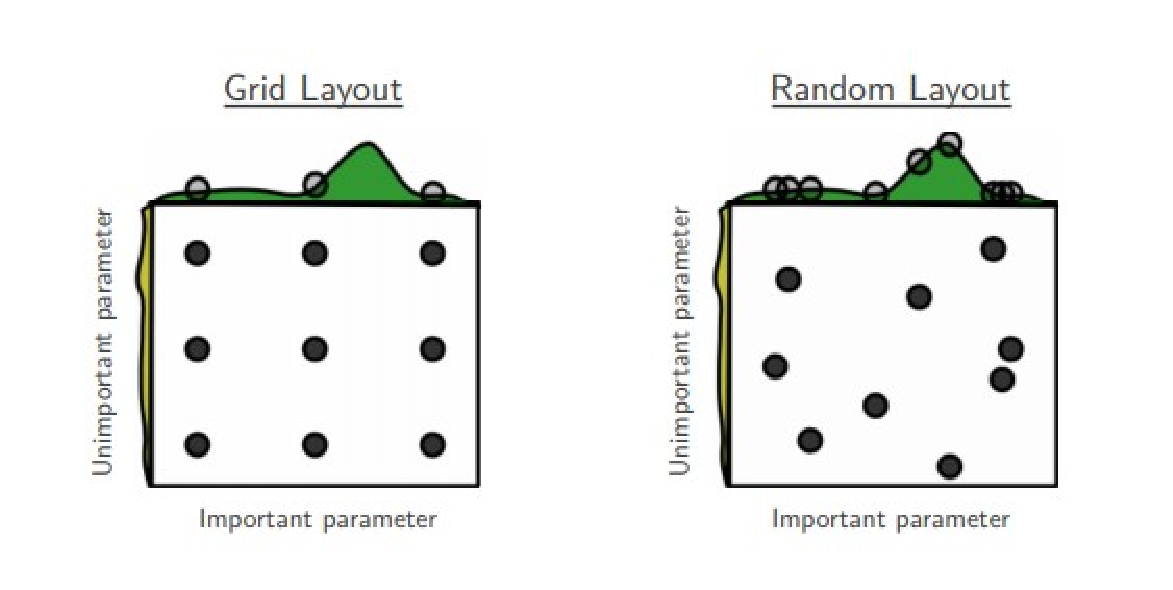
\includegraphics[scale=0.7]{images/chapter_2/random_search.eps}}
\caption{Grid and random search \citep{bergstra2012random}}
\label{fig:Grid and Random Search}
\end{figure}
In Figure \ref{fig:Grid and Random Search} the Grid search and Random search of nine trials are compared for optimising a generic function $f(x, y) = g(x) + h(x)$ where Above each square $g(x)$ is shown in green, and left of each square $h(y)$ is shown in yellow. With grid search, nine trials only test $g(x)$ in three distinct places. With random search, all nine trials explore distinct values of $g$. This failure of grid search is the rule rather than the exception in high dimensional hyper-parameter optimisation.

\subsubsection{Iterative Methods}

In 2011, \citep{bergstra2011algorithms} carried out a state of the art of hyper-parameter optimisation methods for deep neural network models. This work shows the interest of iterative optimisation, based on the criterion of the Expected Improvement of the model performance, proposed by \citep{jones2001taxonomy}. The study introduces two optimisation methods. One method seeks to model the optimisation problem by \textit{Gaussian stochastic processes} (GP) and the second TPE (\textit{Tree-structured Parzen Estimator}) method proposes a kernel-based modelling. These methods are based on the construction of meta-models. The study highlighted the superiority of these two methods over the optimisation by random sampling. In the context of this research work we applied solely the TPE algorithm.

\paragraph{TPE approach} \label{TPE approach}

The Tree-structured Parzen Estimator (TPE) is a sequential model-based optimisation (\textit{SMBO}) approach. SMBO methods sequentially construct models to approximate the performance of hyper-parameters based on historical measurements, and then subsequently choose new hyper-parameters to test based on this model. The TPE approach models $P(x|y)$ and $P(y)$ where x represents hyper-parameters and y the associated quality score. $P(x|y)$ is modelled by transforming the generative process of hyper-parameters, replacing distributions of the configuration prior with non-parametric densities.

In this subsection we have shown how the hyper-parameters can be optimised. Whether it is carried out through a Random sampling approach or through the use of iterative methods, hyper-parameter optimisation is an expensive task in term of computation time. The cost of optimising these models is very high, due to the infinity of possible architectures and the many hyper-parameters, especially for neural networks. In the following subsection, we will present an approach that allows to reduce the overall computational time and which facilitates the convergence of the model, especially if the number of samples composing the training set is not particularly high.


\subsubsection{Transfer Learning} \label{Transfer Learning}

Transfer learning is biologically motivated by the way that humans apply learned knowledge to solve new problems, and consists in exploiting knowledge learned in one problem and searching a good protocol of transferring to a new problem.
In practice, in transfer learning problems, a parametric model is trained in the source problem and transferred to the target problem in a special way, like transferring parameters, or considering the relations between problems. This approach become particularly interesting when we deal with a dataset where the number of samples is small. There is no a well-defined rule to distinguish between a small and a large dataset. Moreover, the amount of data required to solve a machine Learning problem depends on the task that we try to accomplish. In the context of this research project we consider as small, every dataset that have less than 1000 samples. 

Convolutional networks are broadly applicable in the fields mentioned before. The success of transfer learning with convolutional networks relies on the generality of the learned representations that have been constructed from a large database like ImageNet \citep{deng2009imagenet}. \citep{yosinski2014transferable} quantified the transferability of these pieces of information in different layers, e.g. the first layers learn general features, the middle layers learn high-level semantic features and the last layers learn the features that are very specific to a particular task. \citep{zeiler2014visualizing} also visualised the features in the intermediate layers, demonstrating, with images, that convolutional networks learn features from general level to task-specific level. Overall, the learned representations can be conveyed to related but different domains and parameters in the network are reusable for different tasks. The intuition behind transfer learning for image-related tasks is that if a model is trained on a large and general enough dataset, this model will effectively serve as a generic model of the visual world. You can then take advantage of these learned feature maps without having to start from scratch by training a large model on a large dataset.

In practice, we distinguish two successive stages in the training of a neural network by transfer learning: the training of the new last layers, and then the specialisation of the whole network. The first stage is to guarantee the convergence of the classifier on the new task. We seek to obtain a satisfactory inference score. This is why in a first step, only the weights of the neurons of the new last layers are adjusted by back-propagation of the error gradient. Once the convergence of the last layers has been obtained, it is possible to fine-tune the whole network by performing an adjustment of all the weights of the layers in order to improve the classification score.


\section{Conclusion}

In the manufacturing industry, product quality is an indicator for evaluating the production capacity of a company. Customers are increasingly demanding in terms of product quality and providing the customer with a product that complies with the specifications is absolutely essential in a market that is becoming more and more competitive. The best possible solution to deliver 100\% of compliant parts to the customer would be to inspect in details all parts produced. However, most companies cannot test every single product. There may simply be too high a volume or number of them to inspect at a reasonable cost or within a reasonable time frame. Or effective testing might result in the destruction of the product or render it unfit for sale in some way. Moreover, traditional process control approach does not take into account the relationship between process data and produced part quality. In this chapter we have described a general approach that can be applied every time that we want to take advantage of an historical set of data to improve manufactured parts quality. The presented data-driven approach requires 4 main stages: data acquisition, data processing, exploratory data analysis and machine learning modelling. Data acquisition involves the task of identifying all the input process data, as well as the output quality data, that are interesting to try to solve our quality improvement use-case. Data processing is the task of processing and filtering raw input data in order to reduce the noise within data and to make data suitable for Machine Learning modelling. Exploratory data analysis could be used for better understanding the correlation between data and to eventually fine tune the data processing stage. Finally, Machine Learning modelling allows to build a model which relate input process data and output quality data. In such a way it is possible, for a new set of input data, to provide the prediction, or inference of the quality of the finished part. Moreover, using an interpretable model it is possible to identify which process parameters affect the most manufactured parts quality and eventually improve process monitoring. There exists a wide variety of machine learning algorithms. In the second section of this chapter we have presented the linear regression and the linear models with a penalisation term, Tree-Based methods, Support Vector Machines and a few Deep-learning architectures that we have applied all along our research work.

In the following Chapters we will present an application of this method in the industrial context studied along this doctoral studies.


\subsection{Industrial Contribution}

From the industrial point of view, this chapter proposes a new way of looking at process monitoring and quality control. Instead of relying in acceptance sampling method, the historical set of collected data can be leveraged to create an inferring model able to provide a real-time quality inspection without any direct measurement of the part. This would allow for two major benefits:

\begin{itemize}
    \item Faster quality non-conformity detection. In fact, by providing a quality status for each part produced, it is possible to quickly react and adjust the production process to prevent occurrence of new non-conformities.
    \item Destructive tests reduction. If the model is reliable enough to provide accurate results, it is possible to reduce the amount of destructive tests that are regularly performed to assess part quality.
    \item Better comprehension of the production process. If the supervised learning modelling is done through an interpretable Machine Learning algorithm, it is possible to identify which process parameters affect the most part quality. In such a way, it is possible to fine-tune the process by focusing more attention in the control of important parameters. 
\end{itemize}